
%%%%%%%%%%%%%%%%%%%%%%%%%%%%%%%%%%%%%%%%%%%%%%%%%%%%%%%%%%%%%%%%%%%%%%%%%%%%%%%
% Active Learning Machine Learning Methodology %%%%%%%%%%%%%%%%%%%%%%%%%%%%%%%%
% %%%%%%%%%%%%%%%%%%%%%%%%%%%%%%%%%%%%%%%%%%%%%%%%%%%%%%%%%%%%%%%%%%%%%%%%%%%%%
% Outline:
%   * PARAGRAPH 00
%     - General introduction and high-level overview of algorithm
%   * PARAGRAPH 01
%     - Candidate space generation methodology
%   * PARAGRAPH 02
%     - Quick paragraph about structure featurization
%   * PARAGRAPH 03
%     - Iterative AL algorithm procedure
%   * PARAGRAPH 04
%
%
%
%   * There will not be much motivation for our general approach from the intoduction, so this is a good place to more properly layout our arguments
%
% Points to mention:
%   * Active learning frameworks are a means by which to generate the most valuable training data set, on the fly.
%   * The search space of materials is not a continous space but a discrite array of individual structures
%
% TODO:
%%%%%%%%%%%%%%%%%%%%%%%%%%%%%%%%%%%%%%%%%%%%%%%%%%%%%%%%%%%%%%%%%%%%%%%%%%%%%%%


% ████████ ███████ ███    ███ ██████
%    ██    ██      ████  ████ ██   ██
%    ██    █████   ██ ████ ██ ██████
%    ██    ██      ██  ██  ██ ██
%    ██    ███████ ██      ██ ██
% This is good exposition that probably belongs in the introduction

%
% QUESTION Should this be in the introduction
% COMBAK Does the hansen2019atomistic paper really demonstrate structural optimizations? Double check
Active learning frameworks utilizing surrogate models have been demonstrated to successfully speed up materials discovery for alloy nanoparticles \cite{Jennings2019}, structural optimizations \cite{hansen2019atomistic}, and transition-state searches \cite{torres2019low}, as well as adaptive approaches for global optimization \cite{VanDenBossche2018}.
%
% TODO All global optimization papers go here
% TODO Add review paper for GO
Historically, the most common approach to crystal strcuture prediction relied on classical global optimization schemes,
in which the local/global minimum are found via numerical optimization routines that operate within the continious potential energy surface (PES).
%
These methods are fundementally limited by the curse of dimensionality associated with exploring the highly dimensional potential energy surface (PES),
whose degrees of freedoms (and potential number of polymorphs) rises exponentialy with system size.\cite{Stillinger1999}
%
% I'm repeating the same point twice
As such, the global optimization approach is better suited toward smaller systems and doesn't scale efficiently with system size.
%
An alternative approach to GO is to first, define the set of candidate crystal polymorphs, and secondly, search through the static list of candidates with a selection-type algorithm.
%
This approach relies on being able to prepare candidate structures that are likely to be physical and low in energy.
% TODO Find references for various wasys of preparing candidate structures
To date, there have been various techniques to prepare candidate structures, including generating structures randomly, enumerating space groups, etc.
%
Emperically, we know that nature tends to favor symmetric structures, and thus herein, we use construct a dataset candidate structures that leverage this intuition.


% ################################# Paragraph #################################
% %%%%%%%%%%%%%%%%%%%%%%%%%%%%%%%%%%%%%%%%%%%%%%%%%%%%%%%%%%%%%%%%%%%%%%%%%%%%%
% General intro to AL scheme
%
% %%%%%%%%%%%%%%%%%%%%%%%%%%%%%%%%%%%%%%%%%%%%%%%%%%%%%%%%%%%%%%%%%%%%%%%%%%%%%
% | - Paragraph start
%
Here, we present an active learning accelerated methodology for discovering novel and stable crystal polymorphs.
%
Our approach utilizes an active learning framework and makes use of a surrogate-model,
whereby a simple regression model is trained on a set of candidate materials by iteratively and intelligently sampling structures from a candidate set.
%
A high-level overview of algorithm is presented in figure \ref{fig:all_diagram}.
% TODO Add subplot labels to figure 1
There are two primary parts of the algorithm, the first is the generation of the candidate space,
which defines the list of candidate crystal structures to be searched through (\ref{fig:all_diagram}.a).
%
The structures within the candidate space are then transformed into a vectorial representation by a fingerprinting method which encodes the relevent chemical and structural information into a numerical vector,
which can then be directly used by a machine learning regression model.
%
The second part of the algorithm is the iterative search through candidate space via a continiously retrained surrogate model (\ref{fig:all_diagram}.b).
% __|


% ################################# Paragraph #################################
% %%%%%%%%%%%%%%%%%%%%%%%%%%%%%%%%%%%%%%%%%%%%%%%%%%%%%%%%%%%%%%%%%%%%%%%%%%%%%
% CANDIDATE SPACE GENERATION
%
% %%%%%%%%%%%%%%%%%%%%%%%%%%%%%%%%%%%%%%%%%%%%%%%%%%%%%%%%%%%%%%%%%%%%%%%%%%%%%
% | - Paragraph start
The generation of the candidate space is a critical step in the discovery of novel crystal structures for a given system,
since the initial candidate pool determines which structures that can ultimately be discovered, it is imperative to construct candidates that are sufficiently diverse, such that they encompanse as much of the structural diversity in the PES as possible.
%
% TODO PENDING Ask @Ankit for these numbers
% The MP project number should be correct, but the OQMD number might be wrong
% MP{AB2: 2424, AB3: 2341} | OQMD{AB2: 4736, AB3: 28883}
Herein, the structures that comprise the candidate data sets for \IrOtwo and \IrOthree were constructed by mining for \ABtwo and \ABthree structures in the Materials Project\cite{Jain2013} and OQMD\cite{Kirklin2015} databases
(in total 4528 \ABtwo and 23764 \ABthree entries).
%
Structurally redundant systems were then removed via a space-group based structural classification scheme developed by Jain \latin{et al.} \cite{Jain2018},
whereby structural uniqueness is defined by the element-nonspecific stoicheometry (\ABtwo, \ABthree, etc.), spacegroup symmetry and wyckoff positions of the atoms within the unit cell.
%
Imposing structural uniqness reduces the number of entries considerably to 697 and 259 structures for the \ABtwo and \ABthree stoicheometries, respectively;
this is a prime indication of the lack of structural diversity in the OQMD and MP databases.
%
% NUMBER
Furthermore, only bulk structures containing $\leq$ 75 atoms were included in the final candidate pool to reduce the computational expense of the DFT compuations
(further reducing the candidates spaces to 567 and 256 \ABtwo and \ABthree structures respectively).
%
Next, iridum and oxygen were subsituted for the A and B sites, respectively,
this was then followed by a crude isotropic expansion/contraction of the unit cell to accommodate the atomic radii of iridium and oxygen.
%
% NUMBER
Because of the relitively small size of the candidate space, and because we wish to validate our methods fully, we performed bulk relaxations for all 823 structures in the candidate space.
%
See section (SI Bulk polymorph DFT optimization) for further details on the computational methodology used to relax the bulk structures.
%
Of the 823 structures, 736 were able to be fully optimized, while 87, primarily \ABtwo structures were not able to be converged for a variety of convergence issues stemming from highly volumnous and unphysical initial structures.
%
The resulting candidate space was composed of 487 \IrOtwo and 249 \IrOthree structures, all of which have unique space group/Wyckoff combintations, ensuring their structural uniquness.
%
While not particularly large in size, this data set will serve as a proof of concept.
%
In addition, the size of candidate space is sufficiently small that we can tractably optimize the equilibrium structure for the entire dataset with \latin{ab-initio} DFT, thus allowing us to validate the approach in an `after the fact` manner.
% __|


% ################################# Paragraph #################################
% %%%%%%%%%%%%%%%%%%%%%%%%%%%%%%%%%%%%%%%%%%%%%%%%%%%%%%%%%%%%%%%%%%%%%%%%%%%%%
% Short paragraph on featurization method
%
% %%%%%%%%%%%%%%%%%%%%%%%%%%%%%%%%%%%%%%%%%%%%%%%%%%%%%%%%%%%%%%%%%%%%%%%%%%%%%
% | - Paragraph start
%
The candidate data set was featurized using the Voronoi tessellation fingerprinting scheme developed by Ward \latin{et al.} \cite{Ward2017} which produces a 271 length feature vector for each material that is invariant to isotropic expansions/contractions of the lattice and to a degree, insensitive to the exact atomic coordinates of the atoms.
%
% How many columns of the 271 are redundant if stoich and composition are frozen
Herein, we apply our active learning model to the \IrOtwo and \IrOthree spaces separately, because we are interested in the most stable polymorphs at each stoichiometry.
%
Contraining the stoicheometry per application of the AL algorithm further reduces the 271 length  feature vector to 101 non-zero variance features,
significantly reducing the dimensionality of the features.
%
% COMBAK TODO How much of the variance is captured by the PCA analysis
Further dimensionality reduction is achieved via a principle component analysis (PCA) \cite{Tipping1999}, which was used to reduce the remaining 101 features to 11.
% __|


% ################################# Paragraph #################################
% %%%%%%%%%%%%%%%%%%%%%%%%%%%%%%%%%%%%%%%%%%%%%%%%%%%%%%%%%%%%%%%%%%%%%%%%%%%%%
% Active Learning Loop
%
% NOTE This paragraph is a bit long, find way to split into 2
% %%%%%%%%%%%%%%%%%%%%%%%%%%%%%%%%%%%%%%%%%%%%%%%%%%%%%%%%%%%%%%%%%%%%%%%%%%%%%
% | - Paragraph start
%
The active learning algorithm proceeds through iterative generations of ML training, prediction, and acquisition steps that are visualized in figure \ref{fig:iro2_al}.
%
% COMBAK Did I get all of the important features of GP here? @Jose
To start, we utilized Gaussian process (GP) regression with gaussian (or RBF) kernels as implemented in the CatLearn\cite{hansen2019atomistic,CatLearn_Repo} package for atomistic machine learning applications, and used it to train a regression model on a small seed set of DFT formation energies from randomly selected structures in the candidate space.
%
% NOTE I've introduced the aquis. crit. with the GP uncertainty before talking about aquis. in more detail, need to restructure
Herein, we utilized Gaussian process regression because they are highly flexible regression models which have built-in error quantification for each prediction.
%
The model is then used to predict the formation energies of the entire candidate space.
%
This predicted energy landscape is then used to select the next systems to calculate via a aquisition function, which defines a fitness score for each system, and systems that minimize this quantity are then selected.
%
Herein, we use the so-called GP-UCB acquisition function
%
% TODO Should we change the sigma to an uncertainty term? (more precise/direct)
% The name for this kind of acquisition is calld GP-UCB (Upper confidence bound)
% https://www.cse.wustl.edu/~garnett/cse515t/spring_2015/files/lecture_notes/12.pdf
\begin{equation}
    U = \mu - \kappa \sigma,
\end{equation}
%
where $\mu$ and $\sigma$ is the predicted mean and uncertainty of the formation energy,
and $\kappa$ is a free parameter to tune the relative weighting between exploiting low formation energy systems (small $\kappa$) and exploring high uncertainty regions of the candidate space (large $\kappa$).
%
Here, $\kappa$ is set to $1$ which equally weights the energy and uncertainty.
%
In this work we attempt to trade off exploitation and exploration by weighting the predicted formation energy and the associated uncertainty to bias systems that are both low energy and high uncertainty.
%
% TODO N is used into mean number of atoms (FIX)
Once ranked, the N systems that minimize the acquisition function are selected for full DFT calculations, which are included in the training data of subsequent AL generations.
%
Here we chose a bin size (N) of 5, the value of the bin size ($N$) determines how many structures are selected for DFT calculations,
and as such, determines the degree of parallization of the routine.
%
The optimal value of $N$ depends on the computational resources available, as small values of N result in an algorithm that is slow, as every DFT calculation is performed serially.
%
% TODO: Is this statement true?
Larger values of N speed up the active-learning algorithm, but leads to a higher number of DFT calculations performed before convergence.
%
Although initially unique, the structures in the candiate often relax into one another over the course of the DFT optimization, introducing duplicate structures in the post-DFT structures.
%
These duplicate structures are removed during each generation of the AL algorithm, leaving only a single instance of lowest energy in the candidate pool.
%
The coordination characterization function (CCF) based methodology to quantify the simalarity between structures was used to identify and remove duplicate structures.\cite{Su2017}
%
% COMBAK We are discussing alternative convergence criteria, or whether to even have convergence criteria here
The AL loop proceeds until convergence is achieved, which here is chosen to be the generation at which the structures within the range of metastability, here taken as 0.1 eV/atom, are unchanging over three consecutive generations.
% __|



% | - Figure | Active Learning Algorithm **************************************
\begin{figure*}[!htb]
\centering
\makebox[\textwidth][c]{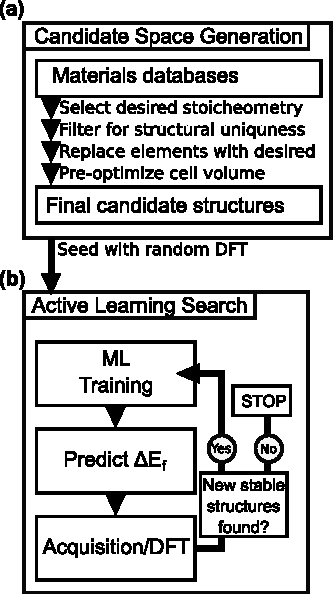
\includegraphics
  {02_figures/al_diagram/Surrogate_model_mine.pdf}
  }
\caption{\label{fig:all_diagram}
% Probably better to keep this caption really concise and refer to the text
Process flow diagram for the active learning accelerated algorithm. The procedure is composed of (a) generation of the candidate set of considered crystal structures constructed from DFT materials databases and (b) iterative active learning surrogate search of the candidate space.
}
\end{figure*}
% __|
